\documentclass{article}

\usepackage{fancyhdr}
\usepackage{extramarks}
\usepackage{amsmath}
\usepackage{amssymb}
\usepackage{enumerate}
\usepackage{graphicx}
\usepackage{braket}
\usepackage{cancel}
\usepackage{pgfplotstable}
\usepackage{listings}

\lstset{framexleftmargin=5mm, frame=shadowbox, rulesepcolor=\color{blue}}

% Useful things
\newcommand{\vcenteredinclude}[1]{\begingroup
\setbox0=\hbox{\includegraphics{#1}}%
\parbox{\wd0}{\box0}\endgroup}

%% better: (general command to vertically center horizontal material)
\newcommand*{\vcenteredhbox}[1]{\begingroup
\setbox0=\hbox{#1}\parbox{\wd0}{\box0}\endgroup}

%
% Basic Document Settings
%

\topmargin=-0.45in
\evensidemargin=0in
\oddsidemargin=0in
\textwidth=6.5in
\textheight=9.0in
\headsep=0.25in

\linespread{1.1}

\pagestyle{fancy}
\lhead{\hmwkAuthorName}
\chead{\hmwkClass\ : \hmwkTitle}
\rhead{\firstxmark}
\lfoot{\lastxmark}
\cfoot{\thepage}

\renewcommand\headrulewidth{0.4pt}
\renewcommand\footrulewidth{0.4pt}

\setlength\parindent{24pt}

%
% Create Problem Sections
%

\newcommand{\enterProblemHeader}[1]{
    \nobreak\extramarks{}{Problem \arabic{#1} continued on next page\ldots}\nobreak{}
    \nobreak\extramarks{Problem \arabic{#1} (continued)}{Problem \arabic{#1} continued on next page\ldots}\nobreak{}
}

\newcommand{\exitProblemHeader}[1]{
    \nobreak\extramarks{Problem \arabic{#1} (continued)}{Problem \arabic{#1} continued on next page\ldots}\nobreak{}
    \stepcounter{#1}
    \nobreak\extramarks{Problem \arabic{#1}}{}\nobreak{}
}

\setcounter{secnumdepth}{0}
\newcounter{partCounter}
\newcounter{homeworkProblemCounter}
\setcounter{homeworkProblemCounter}{1}
\nobreak\extramarks{Problem \arabic{homeworkProblemCounter}}{}\nobreak{}

%
% Homework Problem Environment
%
% This environment takes an optional argument. When given, it will adjust the
% problem counter. This is useful for when the problems given for your
% assignment aren't sequential. See the last 3 problems of this template for an
% example.
%
\newenvironment{homeworkProblem}[1][-1]{
    \ifnum#1>0
        \setcounter{homeworkProblemCounter}{#1}
    \fi
    \section{Problem \arabic{homeworkProblemCounter}}
    \setcounter{partCounter}{1}
    \enterProblemHeader{homeworkProblemCounter}
}{
    \exitProblemHeader{homeworkProblemCounter}
}

%
% Homework Details
%   - Title
%   - Due date
%   - Class
%   - Section/Time
%   - Instructor
%   - Author
%

\newcommand{\hmwkTitle}{Homework\ \#7}
\newcommand{\hmwkDueDate}{March 23, 2015}
\newcommand{\hmwkClass}{PHYS 5243 - Solid State Physics}
\newcommand{\hmwkClassInstructor}{Professor Sheena Murphy}
\newcommand{\hmwkAuthorName}{Chase Brown}


\begin{document}
	\begin{homeworkProblem}
		\textbf{Free Electron Energy in a Square Lattice}
		\hfill

		\begin{enumerate}[(a)]
			\item Show that for a simple square lattice (2D) that the kinetic energy of a free electron in the corner of the first zone is higher than that of an electron a midpoint to a side face of the zone by a factor of 2. 
			\item What is the corresponding factor for a simple cubic lattice in 3D?
			\item What bearing might (b) have on the conductivity of divalent metals?
		\end{enumerate}
		\textbf{Solution}
			\begin{enumerate}[(a)]
				\item The Brillouin Zone for a 2D simple square lattice is shown below:
					\\
					\centerline{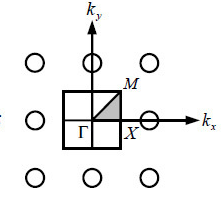
\includegraphics[scale=.5]{SquareBZ2D.png}}
					\\

					Our goal is to show that the energy of an electron at the $M$ point is twice the energy of an electron at the $X$ point. Each side of the BZ is $\frac{4\pi}{a}$, therefore the distance from the $\Gamma$ point to the $X$ point is $\frac{2\pi}{a}$, where as (easily seen by the Pythagorean theorem) the distance between the $\Gamma$ point and the $M$ point is $\sqrt{2}\frac{2\pi}{a}$. So, $\textbf{k}_{X point, 2D} = (\frac{2\pi}{a}, 0)$ and $\textbf{k}_{M point, 2D} = (\frac{2\pi}{a}, \frac{2\pi}{a})$
					
					For a free electron, the eigen energies can be found by starting with the Hamiltonian:
					\begin{equation*}
						H = \frac{\textbf{p}^2}{2m}
					\end{equation*}
					The corresponding energy eigenstates with plane waves $\ket{\textbf{k}}$, have eigenenergies:
					\begin{equation*}
						\epsilon(\textbf{k}) = \frac{\hbar^2 |\textbf{k}|^2}{2m}
					\end{equation*}
					Therefore, plugging in the values for $\textbf{k}$, we see that:
					\begin{equation*}
						\epsilon_{M, 2D}(\textbf{k}) = \frac{\hbar^2 |\frac{2\pi}{a}\sqrt{2}|^2}{2m} = 2\frac{\hbar^2 |\frac{2\pi}{a}|^2}{2m}
					\end{equation*}
					And
					\begin{equation*}
						\epsilon_{X,2D}(\textbf{k}) = \frac{\hbar^2 |\frac{2\pi}{a}|^2}{2m}
					\end{equation*}
					Therefore,
					\begin{equation*}
						\boxed{\epsilon_{M, 2D} = 2\epsilon_{X, 2D}}
					\end{equation*}
				\item Now if we consider this in 3 dimensions, the corner and side get shifted by $\frac{2\pi}{a}$ in one dimension each.  So, $\textbf{k}_{X point, 3D} = (\frac{2\pi}{a}, 0, \frac{2\pi}{a})$ and $\textbf{k}_{M point, 3D} = (\frac{2\pi}{a}, \frac{2\pi}{a}, \frac{2\pi}{a})$.\\
					Therefore we end up with the following eigenenergies:
					\begin{equation*}
						\epsilon_{M, 3D}(\textbf{k}) = \frac{\hbar^2 |\frac{2\pi}{a}\sqrt{3}|^2}{2m}
					\end{equation*}
					And
					\begin{equation*}
						\epsilon_{X, 3D}(\textbf{k}) = \frac{\hbar^2 |\frac{2\pi}{a}\sqrt{2}|^2}{2m}
					\end{equation*}
					Therefore,
					\begin{equation*}
						\boxed{\epsilon_{M, 3D} = \frac{3}{2}\epsilon_{X, 3D}}
					\end{equation*}
				\item This shows that when divalent metals have a band gap which is smaller than the difference in energy between these two points, some electrons will move to the conduction band in order to travel through the material and will threfore become conductive. 
			\end{enumerate}
	\end{homeworkProblem}
	

	\pagebreak
	
	\begin{homeworkProblem}
		\textbf{Free Electron Energies in Reduced Zone Scheme}

		Consider the free electron bands of an FCC crystal lattice in the approximation of an empty lattice but in the reduced zone scheme in which all the $\textbf{K}$s are transformed to lie in the 1st Brillouin Zone.\\

		Plot in the $[111]$ direction the energies of all the bands up to six times the lowest band energy at the zone boundary $\textbf{k}=\frac{2\pi}{a}(\frac{1}{2}, \frac{1}{2}, \frac{1}{2})$. Let this be the unit of energy. \\
		This problem shows why band edges need not neccesarliy be at the zone center.\\
		Several of the degeneracies (band crossings) will be removed when the crystal potential is included.\\
		\hfill
		\\
		\textbf{Solution}

		To start, we look at the reciprocol lattice of the FCC crystal, which is known to be a BCC lattice with lattice constant $\frac{4\pi}{a}$, as shown in Chapter 2 of Kittel's Introduction to Solid State Physics in the subsection "Reciprocol lattice to the FCC lattice" on page 37.  The reciprocol lattice is shown below:
		\\
		\centerline{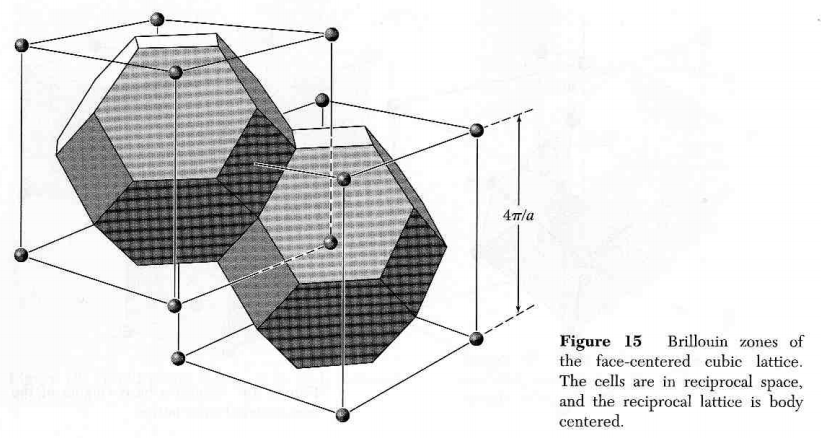
\includegraphics[scale=.5]{ReciprocolFCC.png}}
		\\
		Using the empty lattice approximation and when the free electron model works well, we have:
		\begin{equation*}
			\epsilon(\textbf{k}) = \frac{\hbar^2 |\textbf{k}|^2}{2m}
		\end{equation*}
		Due to the periodicity, under the reduced zone scheme:
		\begin{equation*}
			\textbf{k'} = \textbf{k}+\textbf{G}
		\end{equation*}
		\begin{equation*}
			\Rightarrow \epsilon(k_x, k_y, k_z) = \frac{\hbar^2}{2m}(\textbf{k}+\textbf{G})^2
		\end{equation*}
		$\textbf{G}=0$ for the lowest band.  Therefore,
		\begin{equation*}
			\epsilon(k_x, k_y, k_z) = \frac{\hbar^2}{2m}(k_x + k_y + k_z)^2
		\end{equation*}
		for $[111]$ at the band edge,  $k_x=k_y=k_z=\frac{\pi}{a}$. Therefore,		
		\begin{equation*}
			\epsilon(k_x, k_y, k_z) = \boxed{3\frac{\hbar^2}{2m}(\frac{\pi}{a})^2 = \epsilon_0}
		\end{equation*}
		This value sets the units for the plot, as put in the question.\\
		
		Now with $\textbf{k}=\frac{\pi}{a}(1,1,1)u$ where $u \in [-1,1]$ and $\textbf{G} = m_1 \textbf{b}_1 + m_2 \textbf{b}_2 + m_3 \textbf{b}_3$, we obtain the following equation for the energy of each band normalized to our $\epsilon_0$.
		\begin{equation*}
			\boxed{ \frac{\epsilon(u, \textbf{G})}{\epsilon_0} = \frac{1}{3}[(u+2(-m_1+m_2+m_3))^2 + (u+2(m_1-m_2+m_3))^2 + (u+2(m_1+m_2-m_3))^2] }
		\end{equation*}
		We can then plot the output by creating a simple python script given here:
		\\
		\lstinputlisting[language=Python]{FCCBandStructure111.py}
		\pagebreak
		Which provides the following plot as it's output: \\
		\centerline{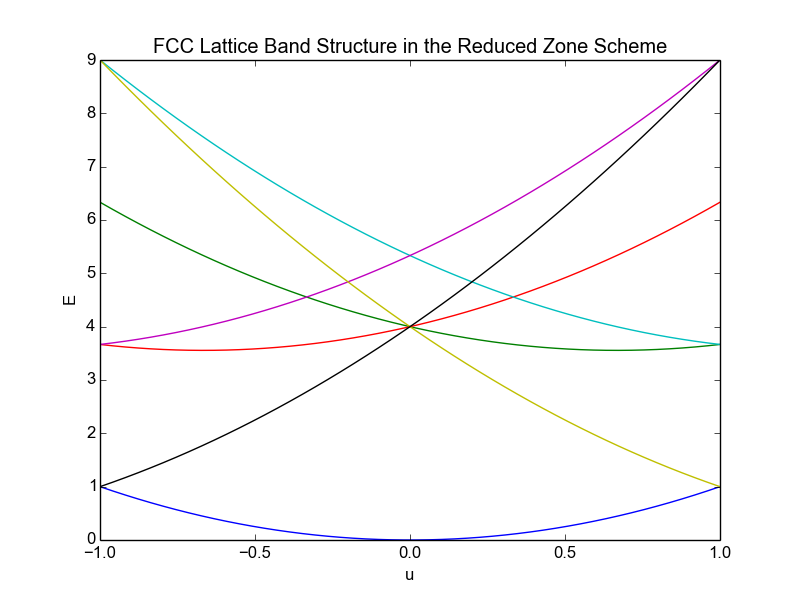
\includegraphics[scale=.5]{FCCBandStructure.png}}
	\end{homeworkProblem}

	\pagebreak
	
	\begin{homeworkProblem}
		\textbf{Kronig-Penny Model Energy and Band Gap (Kittel Chapter 7)}

		\begin{enumerate}[(a)]
			\item Use the Kronig-Penny Model with the delta function with the following values: $P << 1$ and $k = 0$, in order to find the energy of the lowest band.
			\item Find the band gap at $k=\frac{\pi}{a}$.
		\end{enumerate}

		\textbf{Solution}
		
		\begin{enumerate}[(a)]
			\item We start with the solution found for the Kronig-Penny Model in Kittel Chapter 7, Equation 21b:
				\begin{equation*}
					\frac{P}{Ka}sin(Ka) + cos(Ka) = cos(ka)
				\end{equation*}
				Now with $k=0$, we see that $cos(ka)=1$, therefore:
				\begin{equation*}
					\frac{P}{Ka}sin(Ka) + cos(Ka) = 1
				\end{equation*}
				Now, since $P<<1$, and we are interest in the lowest band ($K$ close to zero), we see that $Ka<<1$, therefore we should be interested in the Maclaurin series for cos(x) and sin(x):
				\begin{equation*}
					cos(x) = \sum_{n=0}^{\infty}{\frac{(-1)^n}{(2n)!}x^{2n}} = 1-\frac{x^2}{2!}+\frac{x^4}{4!}+\ldots
				\end{equation*}
				\begin{equation*}
					sin(x) = \sum_{n=0}^{\infty}{\frac{(-1)^n}{(2n+1)!}x^{2n+1}} = x-\frac{x^3}{3!}+\frac{x^5}{5!}+\ldots
				\end{equation*}
				Therefore, we can expand the equation about zero in the Maclaurin series to find that:
				\begin{equation*}
					\frac{P}{Ka} [Ka - \frac{(Ka)^3}{3!} + \frac{(Ka)^5}{5!}+\ldots] + [1 - \frac{(Ka)^2}{2!} + \frac{(Ka)^4}{4!}+\ldots] = 1
				\end{equation*}
				Discounting all but the second order term and assuming the 3rd order and above terms have little effect, we get:
				\begin{equation*}
					\frac{P}{Ka} [Ka - \cancelto{0}{\frac{(Ka)^3}{3!}} + \cancelto{0}{\frac{(Ka)^5}{5!}}] + [1 - \frac{(Ka)^2}{2!} + \cancelto{0}{\frac{(Ka)^4}{4!}}] \approx 1
				\end{equation*}
				\begin{equation*}
					\frac{P}{Ka} [Ka] + [1 - \frac{(Ka)^2}{2!}] \approx 1
				\end{equation*}
				Therefore,
				\begin{equation*}
					P \approx \frac{(Ka)^2}{2!}
				\end{equation*}
				Now since we are interestd in what $K$ is in order to give us the energy by the equation:
 				\begin{equation*}
					\epsilon(\textbf{k}) = \frac{\hbar^2 |\textbf{k}|^2}{2m}
				\end{equation*}
				We find that 
 				\begin{equation*}
					K^2 \approx \frac{2P}{a^2}
				\end{equation*}
				Therefore,
 				\begin{equation*}
					\boxed{\epsilon(\textbf{k=0}) \approx \frac{\hbar^2 P}{ma^2}}
				\end{equation*}

			\item For $k=\frac{\pi}{a}$, we can do a similar approach to the problem. We see that $cos(ka)=-1$ for $k=\frac{\pi}{a}$, and for $P<<1$, $K\approx \frac{\pi}{a}$.\\
				We start again with the Equation from Kittel:

				
				\begin{equation*}
					\frac{P}{Ka}sin(Ka) + cos(Ka) = cos(ka)
				\end{equation*}
				Therefore our expansion around $K=\frac{\pi}{a}$ for  yeilds the following:
				\begin{equation*}
					\frac{P}{\pi+(Ka-\pi)} sin(\pi+(Ka-\pi)) + cos(\pi+(Ka-\pi)) = -1
				\end{equation*}
				Now the expansion becomes:
				\begin{equation*}
					\frac{P}{\pi} [1 - \frac{Ka-\pi}{\pi} +\ldots][-(K-\pi)\ldots] + [-1 - \frac{(Ka-\pi)^2}{2} + \ldots] = -1
				\end{equation*}

				Discounting all but the second order term and assuming the 3rd order and above terms have little effect, we get:
				\begin{equation*}
					K_1 \approx \frac{\pi}{a}
				\end{equation*}
				\begin{equation*}
					K_2 \approx \frac{\pi}{a} + \frac{2P}{\pi a}
				\end{equation*}
				Therefore,
 				\begin{equation*}
					E_g = \epsilon(K_2)-\epsilon(K_1) = \frac{\hbar^2}{2m} [K_2^2-K_1^2]
				\end{equation*}
				Therefore,
 				\begin{equation*}
					\boxed{E_g \approx \frac{2\hbar^2 P}{ma^2}}
				\end{equation*}
		\end{enumerate}


	\end{homeworkProblem}

\end{document}
